\chapterimage{blue25.jpeg} % Imagen de encabezado de capítulo
\chapterspaceabove{6.75cm} % Espacio en blanco desde la parte superior de la página hasta el título del capítulo en las páginas del capítulo
\chapterspacebelow{6.25cm} % Cantidad de espacio en blanco vertical desde el margen superior hasta el comienzo del texto en las páginas de los capítulos

%------------------------------------------------

\chapter{INDUCCIÓN MATEMÁTICA}\label{ch:induccion}

\tcbsidebyside[title=Blaise Pascal,
      sidebyside adapt=left,
      bicolor,
      colback=white,
      colbacklower=jblueinner,
      colframe=jblueleft,
      fonttitle=\bfseries,
      center title,
      fuzzy shadow = {0pt}{-3pt}{-0.5pt}{0.5pt}{black!35},
]{%
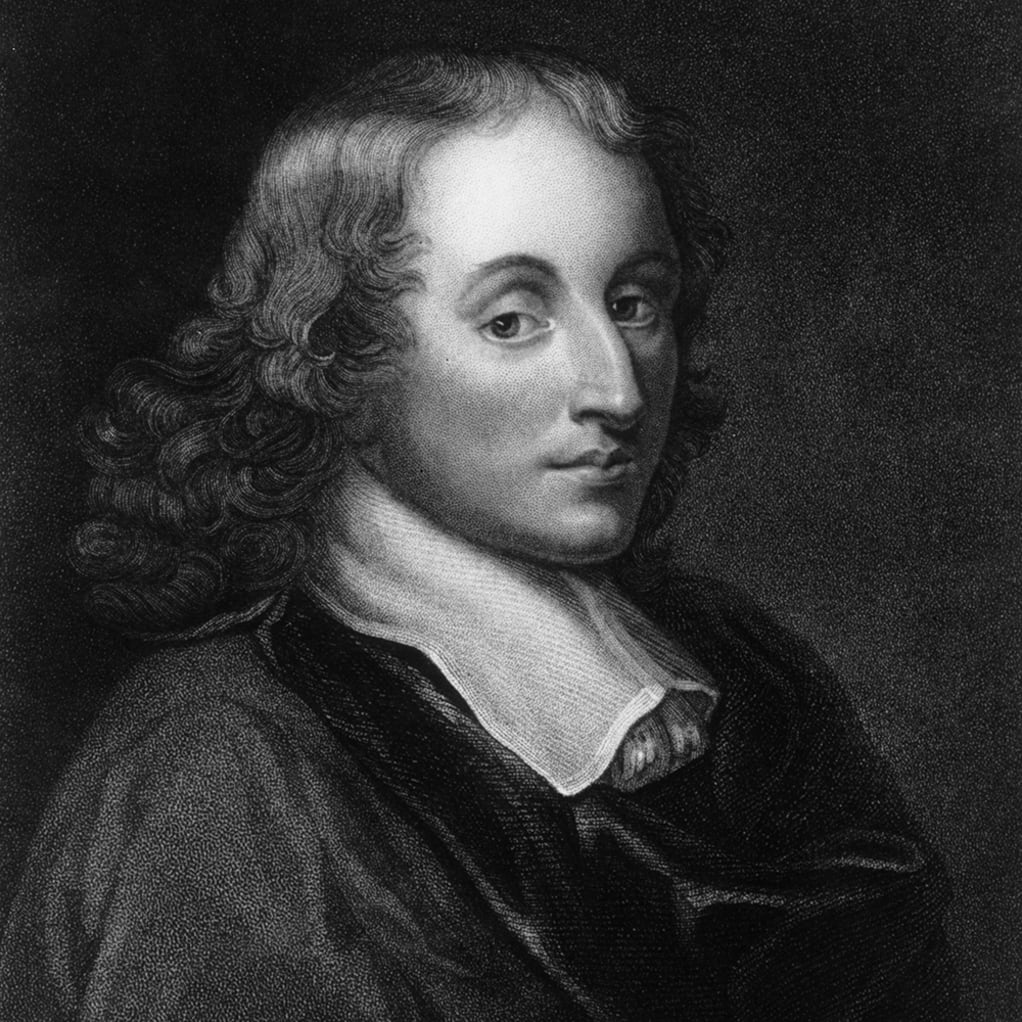
\includegraphics[width=0.36\textwidth]{PASCAL.jpeg}
}{%
    Nacido el 19 de junio de 1623 en Clermont-Ferrand, Francia; fue un genio precoz y de clara inteligencia, pues su entusiasmo juvenil por la ciencia se materializó en importantes y precursoras aportaciones a la física y a las matemáticas. Siendo aún niño, con solo doce años, sin ayuda alguna demostró que la suma de los ángulos de un triángulo es siempre igual a 180°. Su curiosidad lo llevo a que inventara la primera calculadora digital en 1642 (llamada \emph{Pascalina}) para ayudar a su padre, Étienne Pascal. Pese a su frágil salud y corta vida, murió a los treinta y nueve años, pero su huella quedó grabada en la historia de la física y de la informática.
}

%\section{Introducción}

\noindent
\begin{minipage}[c]{0.7\textwidth}
    Uno de los métodos más usados para realizar demostraciones es el Método de Inducción Matemática. Este fue creado por Blaise Pascal en el siglo XVII, aunque el primer matemático que ofreció una demostración formal mediante el uso explicito de la inducción matemática fue el italiano Franciscus Maurolicus (1494-1575). Maurolicus utilizo la inducción para demostrar que para todo entero positivo $n$
    \[1+3+5+\cdots +(2n-1)=n^2.\]
    Dicho método ha servido para demostrar teoremas en distintas áreas de la matemática; como: geometría, teoría de grafos, teoría de números, análisis combinatorio. Una manera informal (pero eficaz) de ver y explicar el Principio de Inducción Matemática es mediante fichas de dominó. Imaginemos que tenemos fichas de dominó puestas en una hilera infinita. Si empujamos la primer ficha, esta empujará la segunda ficha; la segunda ficha empujará la tercer ficha; la tercer ficha empujara la cuarta ficha; y así sucesivamente hasta que caigan \textbf{todas} las fichas. En este caso, cada ficha representa un número natural.
\end{minipage}
\begin{minipage}[c]{0.24\textwidth}
    \noindent
    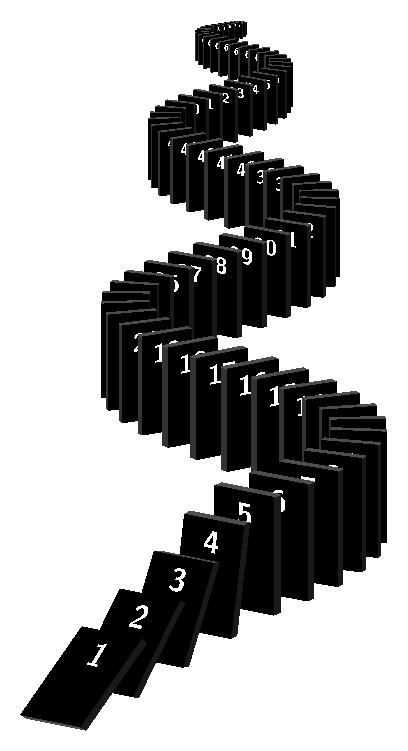
\includegraphics[width=1.17\textwidth]{uuu.pdf}
    %\captionof{figure}{Principio de Inducción}\label{fig:INDUCCION}
\end{minipage}

\newpage

\section{Principio de inducción}

\noindent
\textbf{\color{jblueleft}Problema:} Calcular la suma de los primeros $n$ números impares.\\
\,\\
Los problemas de este tipo se pueden resolver usando una fórmula probada. Pero nos interesa resolver el problema sin recurrir a tal fórmula y aplicando el método de la inducción matemática.
Para hacerlo, es necesario establecer primero una hipótesis, es decir, tratar simplemente de adivinar la solución.\\
\,\\
\textbf{\color{jblueleft}Solución:} Observemos las siguientes sumas parciales:
\begin{align*}
    1 &=1 \\
    1+3 &=4 \\
    1+3+5 &=9 \\
    1+3+5+7 &=16 \\
    1+3+5+7+9 &=25 \\
    1+3+5+7+9+11 &=36 \\
    & \vdots 
    %1+3+5+7+9+11+13 &=49 \\
    %1+3+5+7+9+11+13+15 &=64 %\\
    %1+3+5+7+9+11+13+15+17 &=81
\end{align*}
Cada suma puede representarse en la forma
$$\alpha + \beta + \gamma + \cdots + u = S,$$
donde $u$ representa el último sumando y $S$ la suma. Tanto $u$ como $S$ dependen del número de sumandos, al cual denominaremos con $n$. Dadas estas convenciones podemos hacer las tablas siguientes, y encontrar en la primera de ellas alguna relación entre $n$ y $u$; y en la segunda, alguna relación entre $n$ y $S$.
\begin{center}
    \begin{minipage}[c]{0.2\textwidth}
        \centering
        \begin{NiceTabular}[hvlines-except-borders,rules={color=white,width=1pt}]{cc}
        \CodeBefore
        \rowcolor{jblueleft!80}{1}
        \rowcolors{2}{DodgerBlue3!40}{jblueinner}
        \Body
        \RowStyle[color=white]{}
            $n$ & $u$ \\
            1 & 1 \\
            2 & 3 \\
            3 & 5 \\
            4 & 7 \\
            5 & 9 \\
            6 & 11
            %7 & 13 \\ \hline
            %8 & 15 \\ \hline
            %9 & 9 \\ \hline
        \end{NiceTabular}
    \end{minipage} \hspace{0.3cm}
    \begin{minipage}[c]{0.2\textwidth}
        \centering
        \begin{NiceTabular}[hvlines-except-borders,rules={color=white,width=1pt}]{cc}
        \CodeBefore
        \rowcolor{jblueleft!80}{1}
        \rowcolors{2}{DodgerBlue3!40}{jblueinner}
        \Body
        \RowStyle[color=white]{}
            $n$ & $S$ \\
            1 & 1 \\
            2 & 4 \\
            3 & 9 \\
            4 & 16 \\
            5 & 25 \\
            6 & 36
            %7 & 49 \\ \hline
            %8 & 64 \\ \hline
            %9 & 81 \\ \hline
        \end{NiceTabular}
    \end{minipage}
\end{center}
Por lo que se propone el siguiente modelo:
$$1+3+5+7+9+11+\cdots +(2n-1)=n^2.$$
Probemosla por medio de inducción sobre $n$. Llamemos a la suma, $S_n$. Es decir,
$$S_n=1+3+5+7+9+11+\cdots +(2n-1)$$
\begin{enumerate}[label=\roman*)]
    \item Para $n=1$ es evidente que se cumple, ya que la suma consiste en un solo término, el 1. El valor de la expresión $n^2$ también es 1.
    \item Supóngase que la hipótesis se cumple para $n=k$, es decir, $S_k=k^2$.
    \item A partir de (ii), probemos que se cumple para $n=k+1$, es decir,
    $$S_{k+1}=(k+1)^2.$$
    En efecto, se tiene
    $$S_{k+1}=S_k+(2k+1),$$
    pero $S_k=k^2$. Se sigue que
    $$S_{k+1}=k^2+(2k+1)=(k+1)^2.$$
\end{enumerate}
En conclusión, se cumple que $S_n=n^2$.\\
\newline
Incluso, para este caso, podemos ver la \emph{demostración visual}\footnote{Una demostración visual significa que la solución de dicho problema sea accesible mediante un diagrama o dibujo de forma evidente, sin apenas desarrollo matemático.} de
$$1+3+5+7+9+11+\cdots +(2n-1)=n^2.$$
Imaginemos que cada círculo equivale a una unidad. Entonces,
\begin{enumerate}
    \item Para $n=1$:
    \begin{center}
        \begin{tikzpicture}
            \filldraw[Turquoise1] (0,0) circle (0.25cm);
        \end{tikzpicture}
    \end{center}
    \item Para $n=2$:
    \begin{center}
        \begin{tikzpicture}
            \filldraw[Turquoise1] (0,0) circle (0.25cm);
            \filldraw[jblueleft] (1,0) circle (0.25cm);
            \filldraw[jblueleft] (1,1) circle (0.25cm);
            \filldraw[jblueleft] (0,1) circle (0.25cm);
        \end{tikzpicture}
    \end{center}
    \item Para $n=3$:
    \begin{center}
        \begin{tikzpicture}
            \filldraw[Turquoise1] (0,0) circle (0.25cm);
            \filldraw[jblueleft] (1,0) circle (0.25cm);
            \filldraw[jblueleft] (1,1) circle (0.25cm);
            \filldraw[jblueleft] (0,1) circle (0.25cm);
            \filldraw[SkyBlue1] (2,0) circle (0.25cm);
            \filldraw[SkyBlue1] (2,1) circle (0.25cm);
            \filldraw[SkyBlue1] (2,2) circle (0.25cm);
            \filldraw[SkyBlue1] (1,2) circle (0.25cm);
            \filldraw[SkyBlue1] (0,2) circle (0.25cm);
        \end{tikzpicture}
    \end{center}
    \item Para $n=4$:
    \begin{center}
        \begin{tikzpicture}
            \filldraw[Turquoise1] (0,0) circle (0.25cm);
            \filldraw[jblueleft] (1,0) circle (0.25cm);
            \filldraw[jblueleft] (1,1) circle (0.25cm);
            \filldraw[jblueleft] (0,1) circle (0.25cm);
            \filldraw[SkyBlue1] (2,0) circle (0.25cm);
            \filldraw[SkyBlue1] (2,1) circle (0.25cm);
            \filldraw[SkyBlue1] (2,2) circle (0.25cm);
            \filldraw[SkyBlue1] (1,2) circle (0.25cm);
            \filldraw[SkyBlue1] (0,2) circle (0.25cm);
            \filldraw[RoyalBlue1] (3,0) circle (0.25cm);
            \filldraw[RoyalBlue1] (3,1) circle (0.25cm);
            \filldraw[RoyalBlue1] (3,2) circle (0.25cm);
            \filldraw[RoyalBlue1] (3,3) circle (0.25cm);
            \filldraw[RoyalBlue1] (2,3) circle (0.25cm);
            \filldraw[RoyalBlue1] (1,3) circle (0.25cm);
            \filldraw[RoyalBlue1] (0,3) circle (0.25cm);
        \end{tikzpicture}
    \end{center}
\end{enumerate}
Recordemos que esto es una manera visual de ver el comportamiento de una proposición particular. Pero no siempre se puede recurrir a una demostración visual, ya que nos puede llevar a conclusiones falsas.

\newpage

\begin{tcolorbox}[
      theorem style=change break,
      enhanced,
      breakable,
      boxrule=0pt,
      frame hidden,
      borderline west={3pt}{0pt}{jblueleft},
      colback=jblueinner,
      coltitle=jblueleft,
      attach title to upper={\ },
      sharp corners,
      title={Principio de inducción matemática:},
      fonttitle=\bfseries,
      fontupper=\normalsize
]
    Sea $P$ una propiedad cualquiera. Tenemos que $P(1)$, $P(2)$, $P(3)$, $P(4)$, $\dots$ es un conjunto de propiedades para cada número natural tal que:
    \begin{enumerate}[label=\roman*)]
        \item $P(1)$ es cierta.
        \item Si $P(n)$ es cierta, entonces $P(n+1)$ es cierta.
    \end{enumerate}
    Entonces $P(n)$ es cierta para toda $n \in \mathbb{N}$.
\end{tcolorbox}

\begin{BOX}
    A la suposición de que la propiedad es cierta para $n$ se le conoce como \textbf{hipótesis de inducción} o \textbf{hipótesis inductiva}.
\end{BOX}

\begin{myexample}
    Demostrar que
    $$1+2+\cdots +n=\frac{n(n+1)}{2}, \,\, \forall n \in \mathbb{N}.$$
    
    \tcblower
    \textbf{\color{jblueleft}Demostración:}
    \begin{enumerate}[label=\roman*)]
        \item Claramente $n=1$, satisface la fórmula, ya que
        \begin{align*}
            1 &=\frac{1(1+1)}{2} \\
            1 &=1
        \end{align*}
        \item Supongamos que la fórmula se cumple para $n=k$, es decir, supongamos que
        $$1+2+\cdots +k=\frac{k(k+1)}{2}.$$
        Demostraremos a partir de lo dicho anteriormente que la fórmula se cumple para $n=k+1$. Es decir, probaremos que
        $$1+2+\cdots +k=\frac{(k+1)(k+2)}{2}.$$
        En efecto, por hipótesis de inducción
        $$1+2+\cdots +k=\frac{k(k+1)}{2}.$$
        Entonces
        \begin{align*}
            1+2+\cdots +k+k+1 &=\frac{k(k+1)}{2}+k+1 \\
            &=\frac{k(k+1)+2(k+1)}{2} \\
            &=\frac{(k+1)(k+2)}{2}
        \end{align*}
        es decir,
        $$1+2+\cdots +k+1=\frac{(k+1)(k+2)}{2}$$
    \end{enumerate}
    Por tanto,
    $$1+2+\cdots +n=\frac{n(n+1)}{2}, \,\, \forall n \in \mathbb{N}.$$
\end{myexample}

\begin{BOX}
    Del ejemplo anterior, si utilizamos la notación suma, tenemos:
    $$\sum_{i=1}^n i = 1+2+\cdots +n = \frac{n(n+1)}{2}, \,\, \forall n \in \mathbb{N}.$$
\end{BOX}

\begin{myexample}\label{EX:APUDJSKS}
    Demostrar que
    $$1^2+2^2+\cdots +n^2=\frac{n(n+1)(2n+1)}{6}, \,\, \forall n \in \mathbb{N}.$$
    \tcblower
    \textbf{\color{jblueleft}Demostración:}
    \begin{enumerate}[label=\roman*)]
        \item Claramente $n=1$ satisface la fórmula, ya que al sustituir $n$ por 1 se tiene
        \begin{align*}
            1^2 &=\frac{1(1+1)(2\cdot 1+1)}{6} \\
            1 &=1
        \end{align*}
        lo cual es verdadero.
        \item Supongamos que la fórmula se cumple para $n=k$, es decir, supongamos que
        $$1^2+2^2+\cdots +k^2=\frac{k(k+1)(2k+1)}{6}.$$
        Demostraremos a partir de lo dicho anteriormente que la fórmula se cumple para $n=k+1$. Es decir, probaremos que
        $$1^2+2^2+\cdots +(k+1)^2=\frac{(k+1)(k+2)(2k+3)}{6}.$$
        En efecto: por hipótesis de inducción
        $$1^2+2^2+\cdots +k^2=\frac{k(k+1)(2k+1)}{6}.$$
        Entonces
        \begin{align*}
            1^2 +2^2+\cdots +k^2+(k+1)^2 &=\frac{k(k+1)(2k+1)}{6}+(k+1)^2 \\
            &=\frac{k(k+1)(2k+1)+6(k+1)^2}{6} \\
            &=\frac{(k+1)\big(k(2k+1)+6(k+1)\big)}{6} \\
            &=\frac{(k+1)(2k^2+7k+6)}{6} \\
            &=\frac{(k+1)(k+2)(2k+3)}{6}
        \end{align*}
    \end{enumerate}
    Por tanto,
    $$1^2+2^2+\cdots +n^2=\frac{n(n+1)(2n+1)}{6}, \, \forall n \in \mathbb{N}.$$
\end{myexample}

\newpage

\begin{BOX}
    Del ejemplo anterior, si utilizamos la notación suma, tenemos:
    $$\sum_{i=1}^n i^2 = 1^2+2^2+\cdots +n^2=\frac{n(n+1)(2n+1)}{6}, \, \forall n \in \mathbb{N}.$$
\end{BOX}

\begin{importante}
    El método de la inducción matemática no es el único procedimiento para demostrar que una propiedad $P$ se cumple para cada número natural.
\end{importante}

\begin{BOX}
    En resumen, cuando se quiere demostrar que una propiedad $P$ se cumple para cada número natural, se emplea un procedimiento llamado \textbf{demostración por inducción matemática}. Es decir, si $\mathbb{N}$ es el conjunto de los números naturales y $A \subset \mathbb{N}$ tal que:
    \begin{enumerate}[label=\roman*)]
        \item $1 \in A$.
        \item $k \in A \Longrightarrow k+1 \in A$. Entonces $A=\mathbb{N}$
    \end{enumerate}
\end{BOX}

\begin{importante}
    Si no se puede demostrar que una propiedad $P$ se cumple para cada número natural, no significa que $P$ sea falsa, sino solamente que no se ha podido hacer la demostración. Una manera de demostrar que $P$ es falsa sería dar un \textbf{contraejemplo}.
\end{importante}

\begin{myexample}
    Consideremos el polinomio $f(x)=x^2+x+41$. Si este polinomio se remplaza $x$ por el número 0, se obtiene el número primo 41. Si se remplaza $x$ por el número 1, nuevamente se obtiene un número primo, 43. Si se sigue este procedimiento para 1, 2, 3, 4, 5, 6, 7, 8, 9; obtenemos que
    \begin{align*}
        f(0) &=41 \\
        f(1) &=43 \\
        f(2) &=47 \\
        f(3) &=53 \\
        f(4) &=61 \\
        f(5) &=71 \\
        f(6) &=83 \\
        f(7) &=97 \\
        f(8) &=113 \\
        f(9) &=131
    \end{align*}
    Basándonos en estos resultados podríamos concluir que para todo entero no negativo $x$, el valor del polinomio es un número primo. Pero esto no es así, pues el polinomio $x^2+x+41$ produce números primos para $f(0), \, f(1), \, f(2), \, f(3), \, \dots, \, f(38), \, f(39)$ y al obtener el resultado de $f(40)$, que es $1681$, vemos que es un número compuesto.
\end{myexample}

\newpage

\begin{myexample}
    Demuestre el teorema del binomio. Es decir, $\displaystyle (a+b)^n=\sum_{r=0}^{n}\binom{n}{r}a^{n-r}b^r$.
    
    \tcblower
    \textbf{\color{jblueleft}Demostración:}
    \begin{enumerate}[label=\roman*)]
        \item Si $n=1$, entonces
        \begin{align*}
            \sum_{r=0}^{1}\binom{1}{r}a^{1-r}b^r &= \binom{1}{0} a^{1-0}b^0 + \binom{1}{1} a^{1-1}b^1 \\
            &=a+b
        \end{align*}
        \item Supongamos que se cumple para $n=k$, es decir, supongamos que
        $$(a+b)^k=\sum_{r=0}^{k}\binom{k}{r}a^{k-r}b^r.$$
        Demostraremos a partir de lo dicho anteriormente, que la propiedad se cumple para $n=k+1$, es decir,
        $$(a+b)^{k+1} = \sum_{r=0}^{k+1}\binom{k+1}{r}a^{k+1-r}b^r.$$
        Entonces
        \begin{align*}
            (a+b)^{k+1} &=(a+b)(a+b)^k \\
            &=(a+b) \sum_{r=0}^{k} \binom{k}{r} a^{k-r}b^r \\
            &=a\sum_{r=0}^{k} \binom{k}{r} a^{k-r}b^r + b \sum_{r=0}^{k} \binom{k}{r} a^{k-r}b^r \\
            &=\sum_{r=0}^{k} \binom{k}{r} a^{k+1-r}b^r +  \sum_{r=0}^{k} \binom{k}{r} a^{k-r}b^{r+1} \\
            &=\sum_{r=0}^{k} \binom{k}{r} a^{k+1-r}b^r +  \sum_{r=0}^{k} \binom{k}{r-1} a^{k-(r-1)}b^{r-1+1} \\
            &=\binom{k}{0} a^{k+1} + \sum_{r=1}^{k} \binom{k}{r} a^{k+1-r}b^r + \sum_{r=1}^{k} \binom{k}{r-1} a^{k-r+1}b^r \\
            &= a^{k+1} + \sum_{r=1}^{k} \left[ \binom{k}{r}+\binom{k}{r-1} \right] a^{k+1-r}b^r \\
            &=a^{k+1}+\sum_{r=1}^{k} \binom{k+1}{r} a^{k+1-r} b^r \\
            &=\binom{k+1}{0}a^{k+1-0}b^0+\sum_{r=1}^{k} \binom{k+1}{r} a^{k+1-r}b^r \\
            &=\sum_{r=0}^{k+1} \binom{k+1}{r}a^{k+1-r}b^r
        \end{align*}
    \end{enumerate}
\end{myexample}

\newpage

\begin{myexample}
    Hallar una expresión para la suma
    $$1 \cdot 1! + 2 \cdot 2! + 3 \cdot 3! + \cdots + n \cdot n!.$$
    
    \tcblower
    \textbf{\color{jblueleft}Solución:} Llamemos a la suma anterior, $S_n$. Es decir
    $$S_n=1 \cdot 1! + 2 \cdot 2! + 3 \cdot 3! + \cdots + n \cdot n!.$$
    Veamos las siguientes sumas
    \begin{align*}
        1 \cdot 1! &=1 \\
        1 \cdot 1!+2 \cdot 2! &=5 \\
        1 \cdot 1!+2 \cdot 2! + 3 \cdot 3! &=23 \\
        1 \cdot 1!+2 \cdot 2! + 3 \cdot 3! +4 \cdot 4! &=119 \\
        1 \cdot 1!+2 \cdot 2! + 3 \cdot 3! +4 \cdot 4! +5 \cdot 5! &=719 \\
        & \vdots
    \end{align*}
    Examinando las anteriores sumas, se observa que
    \begin{align*}
        S_1 &=2!-1 \\
        S_2 &=3!-1 \\
        S_3 &=4!-1 \\
        S_4 &=5!-1 \\
        S_5 &=6!-1 \\
        & \vdots
    \end{align*}
    Esto conduce a la hipótesis
    $$S_n=(n+1)!-1.$$
    Verifiquemos dicha hipótesis.
    \begin{enumerate}[label=\roman*)]
        \item La hipótesis se cumple para $n=1$, pues
        $$S_1=1 \cdot 1!=2!-1.$$
        \item Supongamos que la hipótesis se cumple para $n=k$, es decir,
        $$S_k=(k+1)!-1.$$
        En efecto,
        \begin{align*}
            S_{k+1} &= S_k + (k+1) \cdot (k+1)! \\
            &=[(k+1)!-1]+(k+1) \cdot (k+1)! \\
            &=(k+1)![1+(k+1)]-1 \\
            &=(k+1)!(k+2)-1 \\
            &=(k+2)!-1
        \end{align*}
    \end{enumerate}
\end{myexample}